\section{Dataset and Task}

We conduct experiments on two datasets, the details for which are given below.

\subsection{Yelp Service Reviews}

The model is tested on a subset of the Yelp review dataset \citep{challenge2013yelp} and has been sourced from the code repository accompanying the implementation of the paper by \cite{shen2017style} open-sourced by the authors~\footnote{\url{https://github.com/shentianxiao/language-style-transfer}}. It contains 559142, 2000, 2000 sentences for train, validation, and test, respectively, each sampling accompanied by binary sentiment labels. The maximum sentence length is 15, and the vocabulary size is about 9,200.

\subsection{Amazon Product Reviews}

The model is trained and tested on an Amazon product reviews data-set~\footnote{\url{http://jmcauley.ucsd.edu/data/amazon/}}, following \cite{fu2017style}. The reviews were sourced from the code repository accompanying the paper~\footnote{\url{https://github.com/fuzhenxin/text_style_transfer}}. It contains 559142, 2000, 2000 sentences for train, validation, and test, respectively, each sampling accompanied by binary sentiment labels. The maximum sentence length is 20, and the vocabulary size is about 58,000.


\section{Evaluation Metrics}

\subsection{Transfer Strength}

Transfer strength can be defined as a measure of how successful the model has been in generating sentences that are consistent with the attribute the needs to be transferred into them. This can be formulated as a Natural Language Understanding (NLU) task that takes in a sentence as input and predicts the presence of an attribute that we train the model to transfer.

Consistent with the approach taken in \cite{hu2017toward}, \cite{shen2017style} and \cite{fu2017style}, we train a separate model that learns to predict the class among the different classes to which transfer is possible. We use an open source implementation of the work presented by \cite{kim2014convolutional}, which is a convolutional neural network (CNN) model used for text classification, and build it into our model using an open-source implementation as a reference~\footnote{\url{https://github.com/dennybritz/cnn-text-classification-tf}}. This model has frequently been used as a text classification baseline to compare against \citep{tai2015improved} \citep{kiros2015skip} \citep{zhang2015character}.

This CNN classifier is trained on the entire corpus described in the previous section, with a held out validation set to assess improvements in accuracy over time. The test set for this classifier are the style-transferred sentences generated from the autoencoder model.

The style transfer strength is the ratio of sentences successfully transferred to the target style, to the total number of test sentences.
\begin{equation*}
	\text{transfer-strength} = \frac{count(\text{generated sentences with target style attribute})}{count(\text{generated sentences})}
\end{equation*}


\subsection{Content Preservation} \label{ssec:content-preservation-metric}

The content preservation metric used by \cite{fu2017style} is also used in our work to judge content preservation of the generated sentences compared to the original. This metric is needed to ensure that the generated sentence doesn't talk about content, subjects or topics entirely different compared to the original sentence.

This method uses 100-dimensional GloVe embeddings \citep{pennington2014glove} pre-trained on the Wikipedia + GigaWord corpora~\footnote{\url{https://nlp.stanford.edu/projects/glove/}}. The min, mean and max GloVe word embeddings for each sentence are concatenated together to create a sentence representation. The cosine similarity between the source sentence and target sentence is used as a measure of content preservation.

Let $W$ be the set of word embeddings in a sentence $s$. Then the sentence embedding would be given by
\begin{equation*}
	\text{sentence-embedding} = [min(W);max(W);mean(W)]
\end{equation*}

Then the cosine similarity between two sentences $s_1$ and $s_2$ is obtained by
\begin{equation*}
	\text{cosine-similarity} = 1 - \cos(\text{sentence-embedding}_1, \text{sentence-embedding}_2)
\end{equation*}
where $\text{sentence-embedding}_1$ and $\text{sentence-embedding}_2$ are the sentence embeddings for $s_1$ and $s_2$ respectively.

\begin{table}[!t]
	\centering
	\begin{tabular}{| p{0.45\linewidth} | p{0.45\linewidth} |}
		\hline
		\textbf{{Original (Positive)}}                                                      & \textbf{Transferred (Negative)}                  \\
		\hline
		\hline
		we had the shrimp with vegetables and shrimp fried rice both lovely                 & we had the bacon cheeseburger and it was cold    \\
		\hline
		both dishes prepared with quality veggies                                           & eggs benedict with no flavor                     \\
		\hline
		my appetizer was also very good and unique                                          & my steak was very dry and flavorless             \\
		\hline
		both times i have eaten the lunch buffet and it was outstanding                     & yes i have had the worst pizza i have ever had   \\
		\hline
		the new york eggrolls are outstanding and the beef dishes we ordered were flavorful & the main issue was our server was extremely rude \\
		\hline
	\end{tabular}
	\\
	\begin{tabular}{| p{0.45\linewidth} | p{0.45\linewidth} |}
		\hline
		\textbf{{Original (Negative)}}                                        & \textbf{Transferred (Positive)}        \\
		\hline
		\hline
		the chicken '' strip were paper thin oddly flavored strips            & the bread was wonderful as well        \\
		\hline
		the big chicken sandwich should be called the big mayonnaise sandwich & the salsa is the best i have ever had  \\
		\hline
		fries are not worth coming back                                       & prices are good                        \\
		\hline
		but honestly the worst hookah in las vegas                            & very authentic food in the east valley \\
		\hline
		second the service was terribly slow                                  & the sushi was delicious                \\
		\hline
	\end{tabular}
	\caption{Examples of poor content preservation while transferring sentiment}
	\label{tab:poor-content-preservation}
\end{table}

As seen in the examples above, it is easy to optimize for a style-transfer objective as long as there are no constraints on the content preservation regularization. To ensure this does not happen, we typically use a much larger content latent space than style latent space, as well as add the necessary regularizations discussed in the previous chapter.

\subsection{Word Overlap}

\subsection{Cycle Loss}

Cycle loss is not a good metric because while transferring from $X$ to $Y$, and back to $X'$, the variable $Y$ is not observable and if the neural network function is accidentally fitted to transform the content domain, this metric will not be able to tell the difference between an over-fit model and a good model.

\section{Experiment Results}

\subsection{Disentangling Latent Space}

We first analyse how the style (sentiment) and content of the latent space are disentangled. We train a logistic classifier based on different latent spaces, and show results in Table~\ref{tab:classification}.

We see that the 128-dimensional content vector is not discriminative for style. It achieves an accuracy of 0.57, slightly better than random/majority guess. However, the 8-dimensional style vector $\bm s$, despite its low dimensionality, achieves significantly higher style classification accuracy. When combining content and style vectors, we achieve no further improvement. These results verify the effectiveness of our disentangling approach, because the style space does contain style information, whereas the content space doesn't.


\begin{table}
	\centering
	\begin{tabular}{| l | r |}
		\hline
		Random/Majority guess           & 0.5000          \\ \hline
		Content latent space  ($\bm c$) & 0.5690          \\
		Style latent space ($\bm s$)    & \textbf{0.7817} \\
		Combined ($[\bm s;\bm c]$)      & 0.7815          \\
		\hline
	\end{tabular}
	\caption{Style classification accuracy.}
	\label{tab:classification}
\end{table}

\begin{figure}
	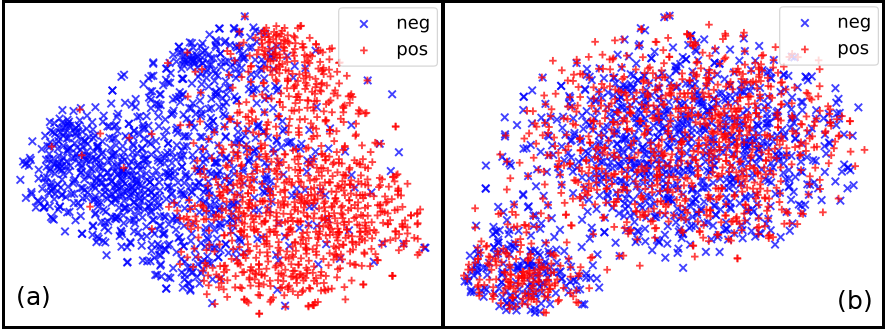
\includegraphics[width=\linewidth]{images/tsne-style-and-content}
	\caption{t-SNE plots of (a) style and (b) content spaces.}
	\label{fig:tsne}
\end{figure}


The latent space can be visualized with t-SNE plots~\cite{maaten2008visualizing} in Figure~\ref{fig:tsne}. As expected, sentences with different sentiments can be nicely separated in the style space (LHS), but are highly mixed in the content space (RHS).


\subsection{Style-Transfer Sentence Generation}

We apply the disentangled latent space to a style-transfer sentence generation task, where the goal is to generate a sentence with different sentiment (style). We followed \cite{fu2017style} and used two metrics: (1) For style transfer, we train a style classifier and predict the accuracy of the generated sentences. While the style classifier itself may not be perfect, it provides a quantitative way of evaluating the strength of style transfer. (2) For the content-preservation score, we compute a sentence embedding by min, max, and average pooling of word embeddings; then a cosine similarity is computed to evaluate how close two sentences are in meaning. Here, sentiment words from a stop list \cite{hu2004mining} are removed.

We compare our approach with state-of-the-art previous work in Table~\ref{tab:comparison-previous}. We re-conducted the experiments with their publicly available code on our data splits.
Results show that, our approach achieves a comparable content-preservation score with previous work, but a significantly better style-transfer score, showing that our disentangled latent space can be used for better style-transfer sentence generation.

Table~\ref{tab:ablation-results} presents the results of an ablation test. We see that both adversarial loss and reconstruction loss play a role in the strength of style transfer, and that they can be combined to further improve performance.

Some examples of style-transfer sentence generation are illustrated in Table~\ref{tab:transfer-samples}. We see that, with the empirically estimated style vector, we can flexibly control the sentiment of generated sentences.

\begin{table}[!t]
	\centering
	\begin{tabular}{| l | r | r | }
		\hline
		\textbf{Model}                        & \textbf{Style Transfer} & \textbf{Content Preservation} \\
		\hline
		\hline
		Cross-alignment \citep{shen2017style} & 0.4609                  & 0.8830                        \\
		\hline
		Sentiment embed. \citep{fu2017style}  & 0.4009                  & 0.9246                        \\
		\hline
		Ours                                  & 0.7708                  & 0.8958                        \\
		\hline
	\end{tabular}
	\caption{Comparison with previous approaches.}
	\label{tab:comparison-previous}
\end{table}


\todo[inline]{Update ablation tests table with latest results}

\begin{table}[!t]
	\centering
	\begin{tabular}{| l | r | r |}
		\hline
		\textbf{Training Loss}                                                        & \textbf{Style Transfer} & \textbf{Content Preservation} \\
		\hline
		\hline
		$\mathcal{L}_\text{rec}$                                                      & 0.5053                  & 0.9103                        \\
		\hline
		$\mathcal{L}_\text{rec}$, $\mathcal{L}_\text{adv}$                            & 0.5901                  & 0.9121                        \\
		\hline
		$\mathcal{L}_\text{rec}$, $\mathcal{L}_\text{mult}$                           & 0.6445                  & 0.9053                        \\
		\hline
		$\mathcal{L}_\text{rec}$, $\mathcal{L}_\text{adv}$, $\mathcal{L}_\text{mult}$ & 0.7708                  & 0.8958                        \\
		\hline
	\end{tabular}
	\caption{Ablation test.}
	\label{tab:ablation-results}
\end{table}


\todo[inline]{Update text samples table with latest results}

\begin{table}[!t]
	\centering
	\begin{tabular}{| p{0.45\linewidth} | p{0.45\linewidth} |}
		\hline
		\textbf{{Original}}                                                        & \textbf{Transferred (Positive $\rightarrow$ Negative)}                    \\
		\hline
		\hline
		i bought this cuisipro mister to replace my old mister last june-(number)  & i bought this a couple of times and was disappointed in this product      \\
		\hline
		quality is good, recevied in time and works as expected.                   & quality is good but i am returning it                                     \\
		\hline
		all in all, i am very happy with this headset.                             & all in all i was expecting a good product                                 \\
		\hline
		\hline
		\textbf{{Original}}                                                        & \textbf{Transferred (Negative $\rightarrow$ Positive)}                    \\
		\hline
		\hline
		i sent it back and requested a refund, and never got the refund.           & i sent it back and gave it a try and it works great                       \\
		\hline
		so i tried just one (number) piece each n still the same results.          & so i bought the two sizes and the other ones are great                    \\
		\hline
		i am going to buy a replacement and wish i had sent this back for a refund & i am going to go through the same time and i have been using it for years \\
		\hline
	\end{tabular}
	\caption{Examples of style-transfer generation.}
	\label{tab:transfer-samples}
\end{table}


\todo[inline]{Add gradually evolving plots of style and content}

\todo[inline]{Juxtapose plots of DAE vs VAE to demonstrate smoothness}

